% !TeX program = pdflatex
\documentclass[aspectratio=169,10pt]{beamer}

\usepackage[utf8]{inputenc}
\usepackage{CJKutf8}
\usepackage{amsmath}
\usepackage{booktabs}
\usepackage{tikz}
\usetikzlibrary{arrows.meta,positioning,shapes.geometric}

\usetheme{Madrid}
\usecolortheme{default}
\hypersetup{bookmarks=false}
\setbeamertemplate{navigation symbols}{}
\setbeamertemplate{footline}[frame number]

\definecolor{lungblue}{HTML}{276EF1}
\definecolor{lungteal}{HTML}{009E8E}
\definecolor{lungorange}{HTML}{E77817}
\definecolor{lungred}{HTML}{CF3F36}
\definecolor{lungink}{HTML}{172033}
\definecolor{lungmuted}{HTML}{596477}
\definecolor{lungbg}{HTML}{F7F8FB}

\setbeamercolor{title}{fg=lungink}
\setbeamercolor{frametitle}{fg=lungink,bg=white}
\setbeamercolor{structure}{fg=lungblue}
\setbeamercolor{normal text}{fg=lungink,bg=white}
\setbeamercolor{block title}{fg=white,bg=lungblue}
\setbeamercolor{block body}{fg=lungink,bg=lungbg}

\setlength{\parskip}{0.25em}
\linespread{1.03}

\newcommand{\code}[1]{\texttt{\small #1}}
\newcommand{\highlight}[1]{\textcolor{lungblue}{\textbf{#1}}}

\tikzset{
  flowbox/.style={
    draw=lungblue!30,
    fill=white,
    rounded corners=2pt,
    minimum height=1.05cm,
    text width=2.05cm,
    align=center,
    font=\small
  },
  smallflowbox/.style={
    draw=lungblue!30,
    fill=white,
    rounded corners=2pt,
    minimum height=0.95cm,
    text width=1.85cm,
    align=center,
    font=\scriptsize
  },
  flowarrow/.style={-Latex,thick,draw=lungblue},
  feedbackarrow/.style={-Latex,thick,draw=lungteal}
}

\title{LungLogic 单肺气流闭环控制}
\subtitle{PID、执行器、Smith Predictor 与校准实验}
\author{Group Meeting}
\date{}

\begin{document}
\begin{CJK*}{UTF8}{gbsn}

\begin{frame}
  \titlepage
\end{frame}

\begin{frame}{本次汇报重点}
  \begin{itemize}
    \item PID 在当前代码中用在哪里？
    \item PID 控制的物理量是什么？
    \item 执行器是什么？
    \item Smith predictor 在闭环中做什么？
    \item PID 需要哪些参数，如何通过实验校准？
    \item Smith predictor 需要哪些参数，如何通过实验校准？
  \end{itemize}

  \vspace{0.8em}
  \begin{block}{核心结论}
    PID 控制的是流量；连续执行器是 PPV40V 比例夹管阀；Smith predictor 只改变 PID 看到的反馈信号，用于补偿气路和传感器延迟。
  \end{block}
\end{frame}

\begin{frame}{当前闭环结构}
  \centering
  \begin{tikzpicture}[node distance=0.45cm]
    \node[smallflowbox] (settings) {Breathing\\settings\\\scriptsize RR, I:E, $V_t$};
    \node[smallflowbox, right=of settings] (ref) {Reference\\flow\\\scriptsize $Q_{\mathrm{ref}}$};
    \node[smallflowbox, right=of ref] (pid) {PID\\controller\\\scriptsize flow error};
    \node[smallflowbox, right=of pid] (ppv) {PPV40V\\valve\\\scriptsize opening};
    \node[smallflowbox, right=of ppv] (plant) {Lung +\\tubing\\\scriptsize plant};
    \node[smallflowbox, right=of plant] (sensor) {SFM3300\\sensor\\\scriptsize flow};

    \draw[flowarrow] (settings) -- (ref);
    \draw[flowarrow] (ref) -- (pid);
    \draw[flowarrow] (pid) -- (ppv);
    \draw[flowarrow] (ppv) -- (plant);
    \draw[flowarrow] (plant) -- (sensor);

    \draw[feedbackarrow] (sensor.south) .. controls +(0,-1.4) and +(0,-1.4) .. node[below,font=\small,text=lungteal] {measured flow 或 Smith-predicted current flow} (pid.south);
  \end{tikzpicture}

  \vspace{1.0em}
  \begin{itemize}
    \item 闭环目标：让测得流量 $Q_{\mathrm{measured}}$ 跟踪目标流量 $Q_{\mathrm{ref}}$。
    \item 体积不是 PID 直接控制量，而是由流量积分得到，并用于阶段终止判断。
  \end{itemize}
\end{frame}

\begin{frame}{PID 在哪里用到}
  \begin{itemize}
    \item Python 仿真：\code{single\_lung\_pid\_gui.py} 中的 \code{PIDController.update()}。
    \item 仿真主循环：\code{run\_single\_lung\_simulation()} 在吸气和呼气阶段调用 PID。
    \item 硬件路径：\code{single\_lung\_hardware\_gui.py} 把 $K_p,K_i,K_d$ 等参数通过 \code{CFG} 发给 STM32。
    \item STM32 固件：\code{updatePID()} 在 100 Hz 控制循环中运行。
    \item 每次状态切换时重置 PID，避免上一个阶段的积分误差带入下一个阶段。
  \end{itemize}

  \vspace{0.4em}
  \begin{block}{PID 控制律}
    \[
      a=\mathrm{clip}\left(
      a_{\mathrm{ff}}+K_p e+K_i\int e\,dt+K_d d,\ 0,\ 1
      \right)
    \]
  \end{block}
\end{frame}

\begin{frame}{PID 控制的是什么}
  \begin{columns}[T,onlytextwidth]
    \begin{column}{0.48\textwidth}
      \begin{block}{被控量}
        \[
          Q_{\mathrm{measured}}\rightarrow Q_{\mathrm{ref}}
        \]
        PID 控制的是 \highlight{流量}，不是压力，也不是直接控制体积。
      \end{block}

      \begin{block}{吸气目标流量}
        \[
          Q_{\mathrm{in,ref}}=0.06\frac{V_{\mathrm{target}}}{T_{\mathrm{fill}}}
        \]
        默认 $250$ mL / $1.30$ s：
        \[
          Q_{\mathrm{in,ref}}=11.54\ \mathrm{SLM}
        \]
      \end{block}
    \end{column}
    \begin{column}{0.48\textwidth}
      \begin{block}{呼气目标流量}
        \[
          Q_{\mathrm{out,ref}}=-0.06
          \frac{V_{\mathrm{target}}}{T_{\mathrm{usable,out}}}
        \]
        PID 实际跟踪负向流量的绝对值。
      \end{block}

      \begin{block}{体积估计}
        \[
          V[k]=V[k-1]+Q[k]\frac{1000}{60}\Delta t
        \]
        体积用于判断是否达到目标潮气量。
      \end{block}
    \end{column}
  \end{columns}
\end{frame}

\begin{frame}{执行器是什么}
  \begin{columns}[T,onlytextwidth]
    \begin{column}{0.48\textwidth}
      \begin{block}{连续控制执行器}
        \begin{itemize}
          \item PPV40V proportional pinch valve
          \item PID 输出归一化开度 $a\in[0,1]$
          \item $a=0$ 表示关闭，$a=1$ 表示全开
        \end{itemize}
      \end{block}

      \begin{block}{电压映射}
        \[
          U_{\mathrm{cmd}}=5(1-a)
        \]
        \[
          a=1 \Rightarrow 0\ \mathrm{V}\ \mathrm{fully\ open}
        \]
        \[
          a=0 \Rightarrow 5\ \mathrm{V}\ \mathrm{fully\ closed}
        \]
      \end{block}
    \end{column}
    \begin{column}{0.48\textwidth}
      \begin{block}{方向选择执行器}
        \begin{itemize}
          \item Atmosphere solenoid valve
          \item Vacuum solenoid valve
        \end{itemize}
      \end{block}

      \begin{block}{状态机控制方向阀}
        \begin{itemize}
          \item Inspiration：大气阀开，真空阀关
          \item Expiration：大气阀关，真空阀开
          \item Dead time：两个方向阀都关
        \end{itemize}
      \end{block}
    \end{column}
  \end{columns}

  \vspace{0.2em}
  \centering
  \highlight{PID 连续调节 PPV40V；电磁阀只负责切换大气/真空气路。}
\end{frame}

\begin{frame}{为什么需要 Smith Predictor}
  \begin{itemize}
    \item 气路传输存在延迟。
    \item SFM3300 传感器和信号处理存在响应滞后。
    \item PID 如果直接使用延迟反馈，可能出现过冲、振荡，或者为了稳定只能调得很慢。
    \item Smith predictor 用模型预测当前流量，再用延迟的真实测量修正模型误差。
  \end{itemize}

  \vspace{0.6em}
  \begin{block}{Smith predictor 反馈估计}
    \[
      Q_{\mathrm{feedback}}
      =
      Q_{\mathrm{model,now}}
      +
      g\left(
      Q_{\mathrm{measured,delayed}}
      -
      Q_{\mathrm{model,delayed}}
      \right)
    \]
  \end{block}

  \vspace{0.2em}
  \centering
  Smith predictor 不替代 PID；它只是给 PID 一个延迟补偿后的反馈流量。
\end{frame}

\begin{frame}{Smith Predictor 在闭环中的位置}
  \centering
  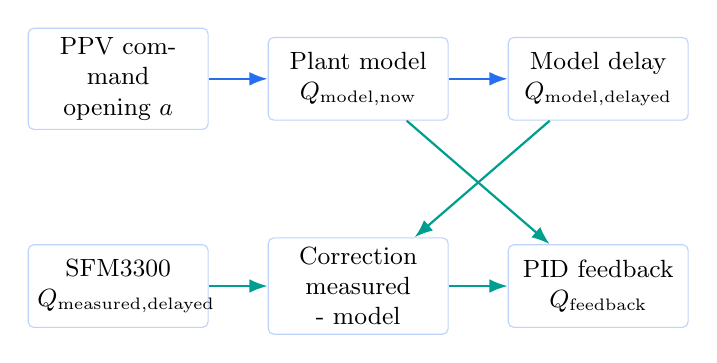
\begin{tikzpicture}[node distance=0.75cm]
    \node[flowbox] (cmd) {PPV command\\opening $a$};
    \node[flowbox, right=of cmd] (model) {Plant model\\$Q_{\mathrm{model,now}}$};
    \node[flowbox, right=of model] (delay) {Model delay\\$Q_{\mathrm{model,delayed}}$};

    \node[flowbox, below=1.45cm of cmd] (sensor) {SFM3300\\$Q_{\mathrm{measured,delayed}}$};
    \node[flowbox, right=of sensor] (corr) {Correction\\measured - model};
    \node[flowbox, right=of corr] (feedback) {PID feedback\\$Q_{\mathrm{feedback}}$};

    \draw[flowarrow] (cmd) -- (model);
    \draw[flowarrow] (model) -- (delay);
    \draw[feedbackarrow] (sensor) -- (corr);
    \draw[feedbackarrow] (delay) -- (corr);
    \draw[feedbackarrow] (model) -- (feedback);
    \draw[feedbackarrow] (corr) -- (feedback);
  \end{tikzpicture}

  \vspace{0.8em}
  \begin{itemize}
    \item 未开启 Smith：PID feedback = measured flow。
    \item 开启 Smith：PID feedback = predicted current flow。
    \item 控制器和执行器不变，变化的是反馈信号。
  \end{itemize}
\end{frame}

\begin{frame}{当前模型参数}
  \begin{columns}[T,onlytextwidth]
    \begin{column}{0.48\textwidth}
      \begin{block}{肺模体与阀门模型}
        \begin{tabular}{ll}
          \toprule
          参数 & 当前初值 \\
          \midrule
          \code{capacity\_ml} & 250 mL \\
          \code{tau\_in\_s} & 0.57 s \\
          \code{tau\_out\_s} & 0.50 s \\
          \code{valve\_exponent} & 1.15 \\
          \code{transport\_delay\_s} & 0.025 s \\
          \code{sensor\_tau\_s} & 0.020 s \\
          \code{sensor\_noise\_slm} & 0.10 SLM \\
          \code{flow\_sign} & 1 \\
          \bottomrule
        \end{tabular}
      \end{block}
    \end{column}
    \begin{column}{0.48\textwidth}
      \begin{block}{PID 参数}
        \begin{tabular}{ll}
          \toprule
          参数 & 当前初值 \\
          \midrule
          $K_p$ & 0.022 \\
          $K_i$ & 0.16--0.21 \\
          $K_d$ & 0.0 \\
          integral limit & 2.0 \\
          control period & 0.01 s \\
          \bottomrule
        \end{tabular}
      \end{block}

      \begin{block}{Smith 参数}
        \begin{tabular}{ll}
          \toprule
          参数 & 当前初值 \\
          \midrule
          enabled & false by default \\
          delay & 0.025 s \\
          correction gain & 0.85--1.0 \\
          \bottomrule
        \end{tabular}
      \end{block}
    \end{column}
  \end{columns}

  \vspace{0.2em}
  \centering
  这些目前应视为仿真和早期硬件调试初值，需要通过台架实验重新辨识。
\end{frame}

\begin{frame}[shrink=5]{PID 需要哪些参数}
  \begin{columns}[T,onlytextwidth]
    \begin{column}{0.48\textwidth}
      \begin{block}{PID 控制器参数}
        \begin{itemize}
          \item $K_p$：比例增益
          \item $K_i$：积分增益
          \item $K_d$：微分增益
          \item integral limit：积分限幅
          \item $\Delta t$：控制周期
        \end{itemize}
      \end{block}
    \end{column}
    \begin{column}{0.48\textwidth}
      \begin{block}{前馈模型参数}
        \begin{itemize}
          \item $V_{\max}$：有效容量
          \item $\tau_{\mathrm{in}}$：吸气时间常数
          \item $\tau_{\mathrm{out}}$：呼气时间常数
          \item $\gamma$：阀门非线性指数
        \end{itemize}
      \end{block}
    \end{column}
  \end{columns}

  \vspace{0.4em}
  \begin{block}{前馈开度}
    \[
      a_{\mathrm{ff}}=
      \left(\frac{Q_{\mathrm{ref}}}{Q_{\max}}\right)^{1/\gamma}
    \]
    \[
      Q_{\max,\mathrm{in}}=0.06\frac{V_{\max}-V}{\tau_{\mathrm{in}}},
      \quad
      Q_{\max,\mathrm{out}}=0.06\frac{V}{\tau_{\mathrm{out}}}
    \]
  \end{block}
\end{frame}

\begin{frame}[shrink=5]{PID 参数校准实验}
  \begin{enumerate}
    \item \textbf{开环 PPV 阶跃实验}
      \begin{itemize}
        \item 固定 PPV 开度：20\%, 40\%, 60\%, 80\%, 100\%。
        \item 分别测试吸气和呼气。
        \item 记录流量、积分体积和响应时间。
      \end{itemize}

    \item \textbf{闭环 PI 调参}
      \begin{itemize}
        \item 先设 $K_d=0$。
        \item 从小 $K_p$ 开始增加，使响应变快但不过度振荡。
        \item 再增加 $K_i$，消除稳态误差和体积误差。
      \end{itemize}

    \item \textbf{多工况验证}
      \begin{itemize}
        \item 测不同 RR、I:E、target volume、target fill time。
        \item 比较 rise time、overshoot、steady-state error、tidal volume error。
      \end{itemize}
  \end{enumerate}
\end{frame}

\begin{frame}{Smith Predictor 需要哪些参数}
  \begin{columns}[T,onlytextwidth]
    \begin{column}{0.48\textwidth}
      \begin{block}{Smith 自身参数}
        \begin{itemize}
          \item $L$ 或 \code{delay\_s}：总延迟
          \item $g$ 或 \code{correction\_gain}：修正增益
          \item \code{enabled}：是否启用 Smith predictor
        \end{itemize}
      \end{block}

      \begin{block}{最关键参数}
        \[
          L =
          t_{\mathrm{flow\ response}}
          -
          t_{\mathrm{command}}
        \]
        即命令变化到传感器测得流量变化之间的延迟。
      \end{block}
    \end{column}
    \begin{column}{0.48\textwidth}
      \begin{block}{运行时需要的信号}
        \begin{itemize}
          \item 当前 PPV 开度 $a$
          \item 当前气路方向：吸气 / 呼气 / 关闭
          \item 传感器延迟测量 $Q_{\mathrm{measured,delayed}}$
          \item 模型当前预测 $Q_{\mathrm{model,now}}$
          \item 模型延迟预测 $Q_{\mathrm{model,delayed}}$
        \end{itemize}
      \end{block}

      \begin{block}{修正增益含义}
        $g=0$：完全相信模型。

        $g=1$：完整加入延迟测量误差修正。

        $g$ 太大可能放大噪声或模型误差。
      \end{block}
    \end{column}
  \end{columns}

  \vspace{0.2em}
  \centering
  注：Smith predictor 内部沿用前面已经介绍过的一阶肺模型，不在本页重复列模型参数。
\end{frame}

\begin{frame}[shrink=5]{Smith Predictor 校准实验}
  \begin{enumerate}
    \item \textbf{延迟辨识实验}
      \begin{itemize}
        \item 给 PPV 开度阶跃。
        \item 同步记录命令时间戳、阀门电压、SFM3300 流量。
        \item 测命令变化到流量明显变化的时间，得到 \code{delay\_s}。
      \end{itemize}

    \item \textbf{模型延迟对齐实验}
      \begin{itemize}
        \item 用拟合模型生成 $Q_{\mathrm{model,now}}$。
        \item 将模型输出延迟 $L$，得到 $Q_{\mathrm{model,delayed}}$。
        \item 与实测 $Q_{\mathrm{measured}}$ 对齐比较。
      \end{itemize}

    \item \textbf{Smith on/off A-B test}
      \begin{itemize}
        \item 保持控制参数、呼吸参数和硬件状态不变。
        \item 分别关闭/开启 Smith predictor。
        \item 比较过冲、振荡、到达目标体积时间和潮气量误差。
      \end{itemize}
  \end{enumerate}
\end{frame}

\begin{frame}{实机迁移前的基础校准}
  \begin{itemize}
    \item \textbf{SFM3300 零点校准}：所有阀关闭，估计零流量 offset 和噪声。
    \item \textbf{流量方向校准}：打开大气路径和真空路径，确认吸气/呼气符号，设置 \code{flow\_sign}。
    \item \textbf{PPV40V 电压--流量映射}：输入多个电压，测稳态流量，确认 $0$ V 全开、$5$ V 全关。
    \item \textbf{吸气阶跃响应}：拟合 $\tau_{\mathrm{in}}$ 和 $\gamma$。
    \item \textbf{呼气阶跃响应}：拟合 $\tau_{\mathrm{out}}$，同时确认真空调压范围。
    \item \textbf{安全验证}：急停、超流量保护、串口 watchdog、方向阀互锁。
  \end{itemize}
\end{frame}

\begin{frame}{汇报总结}
  \begin{itemize}
    \item PID 用在流量闭环中。
    \item PID 控制的是 SFM3300 测得的流量，使其跟踪 $Q_{\mathrm{ref}}$。
    \item PID 输出 PPV40V 比例夹管阀开度。
    \item 电磁阀只负责选择大气或真空气路。
    \item Smith predictor 用模型预测当前流量，并用延迟测量修正模型误差。
    \item PID 校准重点：$K_p,K_i,K_d$、积分限幅和前馈模型参数。
    \item Smith 校准重点：总延迟、修正增益和开启/关闭对比效果。
  \end{itemize}

  \vspace{0.6em}
  \begin{block}{一句话}
    State machine chooses pneumatic direction; PID modulates PPV opening; Smith predictor improves feedback timing.
  \end{block}
\end{frame}

\end{CJK*}
\end{document}
